\documentclass{article}

\usepackage{listings}
\usepackage{graphicx}

\title{Organización de Archivos y Control de Concurrencia sobre una base de datos relacional de crímenes en Boston}
\author{Sebastián Hurtado \and Diego Linares \and Piero Marini}
\date{Septiembre 26, 2019}

\begin{document}
  
  \maketitle

  \section{Introducción}
    
    \subsection{Objetivo del Proyecto}
      
      La meta del presente trabajo es, en una base de datos relacional, desarrollar y probar el funcionamiento de algoritmos de almacenamiento de archivos en memoria secundaria y manejo de concurrencia. Para ello, se hizo uso de un set de data de crímenes en la ciudad de Boston, Massachusets. Sobre esta se implementaron las siguientes tres técnicas de almacenamiento:
      \begin{itemize}
        \item Random File Access
        \item Static Hashing
        \item Dynamic Hashing
      \end{itemize}
      Se realizaron, por medio de transacciones, pruebas del performance de cada una de las implementaciones para observar las mejoras tanto en tiempo de retribución, como en cantidad de accesos a disco. Se emulo así mismo, el funcionamiento de concurrencia a través de threads. 
    
    \subsection{Definiciones previas}  
      
      \subsubsection{Organización de Archivos}
      
        Definimos a un archivo como una colección de registros que se encuentra almacenado en algún tipo de memoria secundaria (discos magnéticos, cintas, etc.). Debido a que la velocidad de acceso a esta memoria se encuentra limitado, es necesario una forma de recuperar estos datos de forma eficiente. La organización de archivos se refiere a la relación entre los registros que los conforman. El objetivo de este es aumentar la eficiencia en términos de la identificación y acceso a un registro en particular. Dependiendo de la \textbf{estructura} en particular utilizada para controlar los registros en forma lógica, es que se obtienen diferentes beneficios para las operaciones de búsqueda, inserción, actualización y borrado.
      
      \subsubsection{Acceso a Archivos} 
        
        Como resultado de la cantidad de información, esta no se puede encontrar en memoria principal para ser trabajada completamente en simultáneo. Por lo tanto, se tiene que acceder archivos individuales, y esto puede ser realizado en una variedad de maneras:

        \begin{itemize}
          
         \item \textbf{Acceso Secuencial}: forma más común de acceso a memoria en la que se accede a los registros uno detrás de otro. Sin embargo, posee altos costos de lectura debido a que se tiene que recorrer linearmente el archivo. La escritura se puede hacer de forma más sencilla si es que se trabaja con una estructura de tipo \textit{heap}.
         
         \item \textbf{Acceso Directo}: permite la lectura y escritura rápida de los archivos que no se encuentran en un orden particular. Se accede de forma directa a un bloque en el disco del cual se extrae la data. No tiene restricciones de orden para sus operaciones.
         
         \item \textbf{Secuencial Indexado}: se construye un índice para el archivo de forma que se puede acceder a cada uno de los bloques de este. Para encontrar un archivo, entramos en el índice a través del cual se puede acceder directamente. 

        \end{itemize}

        En el proceso de este trabajo repasaremos cada uno de estos métodos en las diferentes organizaciones implementadas.

      \subsubsection{Hashing} 
        
        Se refiere al uso de una función de hash para transformar un registro de tamaño arbitrario a un campo de tamaño fijo. La función en cuestión recibe una llave como input que sirve para identificar al registro. El output de la función es un código hash que permite ubicar la data en una tabla de hash que contiene la información correspondiente. Las ventajas que provee se caracterizan tanto por ser en espacio de almacenamiento y en recuperación de data. Por un lado, evita el crecimiento exponencial de espacio de almacenamiento necesario conforme aumenta el número de llaves, mientras que por otro lado los datoos pueden ser obtenidos en un tiempo reducido casi constante - comparado con los tiempos lineares que requieren otras formas de almacenamiento -.

    \subsection{Descripción del dominio de datos y planteamiento del problema} 
      
      El dominio de datos que se seleccionó para este proyecto es un resumen de dominio público sobre crímenes ocurridos en la ciudad de Boston entre 2015 y 2018. De acuerdo a la descripción del mismo: \textit{"este contiene registros del nuevo sistema de reporte de incidentes, que incluye un set reducido de campos enfocado en capturar el tipo de incidente, así como cuando y donde ocurrió"}. Con el objetivo de facilitar el trabajo, se ha reducido la tabla para usar los siguientes campos:

      \begin{center}
      \begin{tabular}{| c | c |}
      
        \hline
        \textbf{Campo} & \textbf{Tipo de Dato} \\
        \hline
        Incident Number & \texttt{char[10]} \\
        Offense Code & \texttt{char[5]} \\
        District & \texttt{char[4]} \\ 
        Reporting Area & \texttt{int} \\
        Shooting & \texttt{char} \\
        Year & \texttt{int} \\
        Month & \texttt{int} \\
        Day of Week & \texttt{char[10]} \\
        Hour & \texttt{int} \\
        UCR Part & \texttt{char[20]} \\
        Street & \texttt{char[20]} \\
        \hline

      \end{tabular}
      \end{center} 

      El problema presente en la base de datos a trabajar es el mal planteamiento de algunos de los campos y las formas de acceso a este a través de un archivo \texttt{.csv}. Los datos originales no se encontraban limpios y poseían campos redudantes y de difícil \textit{parsing} que podían ser mejorados. Además, la llave primaria original se encuentra asignada a un valor binario, "shooting", que únicamente podía ser positivo o negativo. Por otra parte, el tener los archivos almacenados en un único \texttt{.csv} permitía únicamente técnicas de acceso secuenciales. A pesar de la simplicidad de la implementación, la búsqueda e inserción de nueva data era lenta y requería cargar todo el archivo en memoria primaria.

    \subsection{Resultados a obtener} 

      Se espera obtener mejoras en la performance de las instrucciones de inserción y búsqueda en la base de datos relacional y un control de concurrencia mínimo. Para ello, se están implementando 3 diferentes formas de organización de datos las cuales van a ser comparadas con el mismo proceso en la base de datos original. El control de concurrencia será probado a través de transacciones trabajadas en simultáneo utilizando thread control de unix. Se espera que estas realicen una organización serializable que pueda ser aplicada en los diferentes sistemas de organización de archivos.

  \section{Fundamento y descripción las técnicas} 

    \subsection{Descripción de las técnicas}

      \subsubsection{Random File Access}

        En esta técnica los registros en el archivo no requieren ser almacenados secuencialmente. Para mantener la relación entre la llave (en este caso, el Incident Number) y la ubicación del registro en memoria secundaria. La llave es utilizada a través de una función hashing para encontrar la ubicación del registro. Sus ventajas se basan en inserciones y búsquedas eficientes, además de poder mantener el diccionario en todo momento en memoria principal. Su desventaja es el espacio que requiere el mantener este diccionario y las colisiones que pueden ocurrir dependiendo de la función utilizada.

      \subsubsection{Static Hashing}
        
        Se tiene un bucket de registros sobre los cuales la función de hash indica a la cual se dirige uno. La cantidad máxima de entradas en el bucket no varía, por lo que la función siempre calcula la misma dirección. Debido a la cantidad de colisiones que esto puede producir se maneja el overflow a través del desbordamiento encadenado. En este se tiene una lista de buckets adicionales y un puntero al final de cada uno que me indica a cual me debo dirigir en caso este lleno.

      \subsubsection{Dynamic (Extendible) Hashing}

        Usado en base de datos que varían tamaño a través del tiempo. La función hash genera una secuencia de bits, del cual solo se usa un sufijo o prefijo del binario para indexar los registros. Cada bucket tiene una profundidad local que indica cuantos bits se están tomando. Esta técnica evita que la base de datos se degrade con el tiempo y minimiza los casos de overflow. Por otro lado, el cambio de tamaño de buckets es una operación cara y no soporta búsquedas por rango.

    \subsection{Aspectos importantes de la implementación}
        
      \subsubsection{Preparación de la data} 
        
        Como parte del pre-procesamiento de la información previo a cada una de las técnicas de organización se realizaron los siguientes procesos: 

        \begin{itemize}

          \item \textbf{Carpetas y Metadata:} Debido a la cantidad de archivos creados por cada una de las pruebas de las técnicas de almacenamiento, fue necesario la creación de carpetas para cada uno de los buckets a generarse. Además debido al uso de la técnica de \textit{desbordamiento encadenado}, es necesario guardar información tal como el \texttt{top bucket} y el \texttt{index} en memoria secundaria de forma que estos puedan ser cargados antes de cada uso del programa. Esto puede ser observado en las clases \texttt{StaticHash.h} y \texttt{DynamicHash.h}. 

          \item \textbf{Limpieza y Generación Aleatoria:} La base de datos original poseía diversos campos sobre los cuales era díficil hacer parsing, y otros que se encontraban mal parseados en su totalidad (como es el caso de "Shooting"), por lo cual fue necesario reducir el tamaño de la tabla antes de su uso a los 11 campos considerados de mayor importancia. Para las pruebas de inserción y búsqueda de archivos individuales se creo una función \texttt{setLazy()} para generar registros aleatorios con mínimos cambios entre estos.

        \end{itemize}

      \subsubsection{FileOrganization.h}
      
        Archivo que contenía la estructura \texttt{Bucket} y la clase base para la implementación de las técnicas de organización de archivos, la cual toma la siguiente forma. 

        \begin{lstlisting}[language=C++]
        
          #define B 10
          struct Bucket {
            int next;
            int size;
            char *key [B];
            long pos [B];
          };

          template <class T>
          class FileOrganization {
            public:
              virtual void readIndex() = 0;
              virtual void writeIndex() = 0;
              virtual void scan() = 0;
              virtual void insertion(T record) = 0;
              virtual void search(T record) = 0;
          };

        \end{lstlisting}
        
        Este contiene las funciones básicas que fueron implementadas en cada una de las técnicas. 

      \subsubsection{Técnicas de Organización} 
        
        La implementación de cada una de las técnicas fue realizada utilizando conceptos de programación genérica (uso de templates), y la implementación de cada una de las funciones listadas. La función de hasheo utilizada fue utilizar el módulo de la profundidad de los buckets presentes. La implementación de cada una de las funciones para cada una de las técnicas puede ser observada en el repositorio de GitHub del proyecto.

    \subsection{Manejo de Memoria Secundaria}

      El manejo de memoria secundaria se puede ver en el uso de metadata y buckets en forma de archivos que se guardan en el disco duro al momento de correr el programa. Para la creación de un objeto que va a realizar cada una de las técnicas de organización es necesario la lectura de un archivo que se encuentra en memoria secundaria. La creación de buckets y su guardado también se realiza en memoria secundaria, por lo cual hay carpetas designadas para cada uno de estos. Como prueba del software funcionando apropiadamente, vemos la generación de nuevos archivos en cada uno de las carpetas designadas. El programa además, a diferencia de uno que solo funciona en memoria primaria, es que puede ser utilizado varias veces sin pérdida de información gracias al uso de "metadata" en forma de archivos adicionales.

    \subsection{Simulación de Transacciones}

      Las transacciones fueron simuladas en forma de funciones que realizaban un cierto número de operaciones de inserción y búsqueda utilizando un mismo tipo de técnica de organización, y para el control de concurrencia se utilizaron hilos que realizaban estas funciones en simultáneo. Se hizo una variedad de transacciones para cada una de las pruebas. Su funcionamiento correcto se comprobo invocándolas sobre un conjunto de archivos ya existentes para ver que se ejecutaran apropiadamente. Un conjunto de indicadores en forma de texto se utilizaron para observar el orden en el que ocurrieron cada una de las operaciones. Se esperaba obtener una planificación serializable al momento de llevar a cabo las transacciones a través de hilos.

  \section{Resultados Experimentales}

    Para la evaluación del funcionamiento de la aplicación, se uso la función de generación de elementos aleatorios para crear los registros que se iban a insertar en los archivos, y se tomaron los tiempos respectivos de las operaciones de inserción y búsqueda.

    \subsection{Cuadros Comparativos}

      Se tienen 2 cuadros comparativos a mostrar.
    
      \begin{figure}[h]

        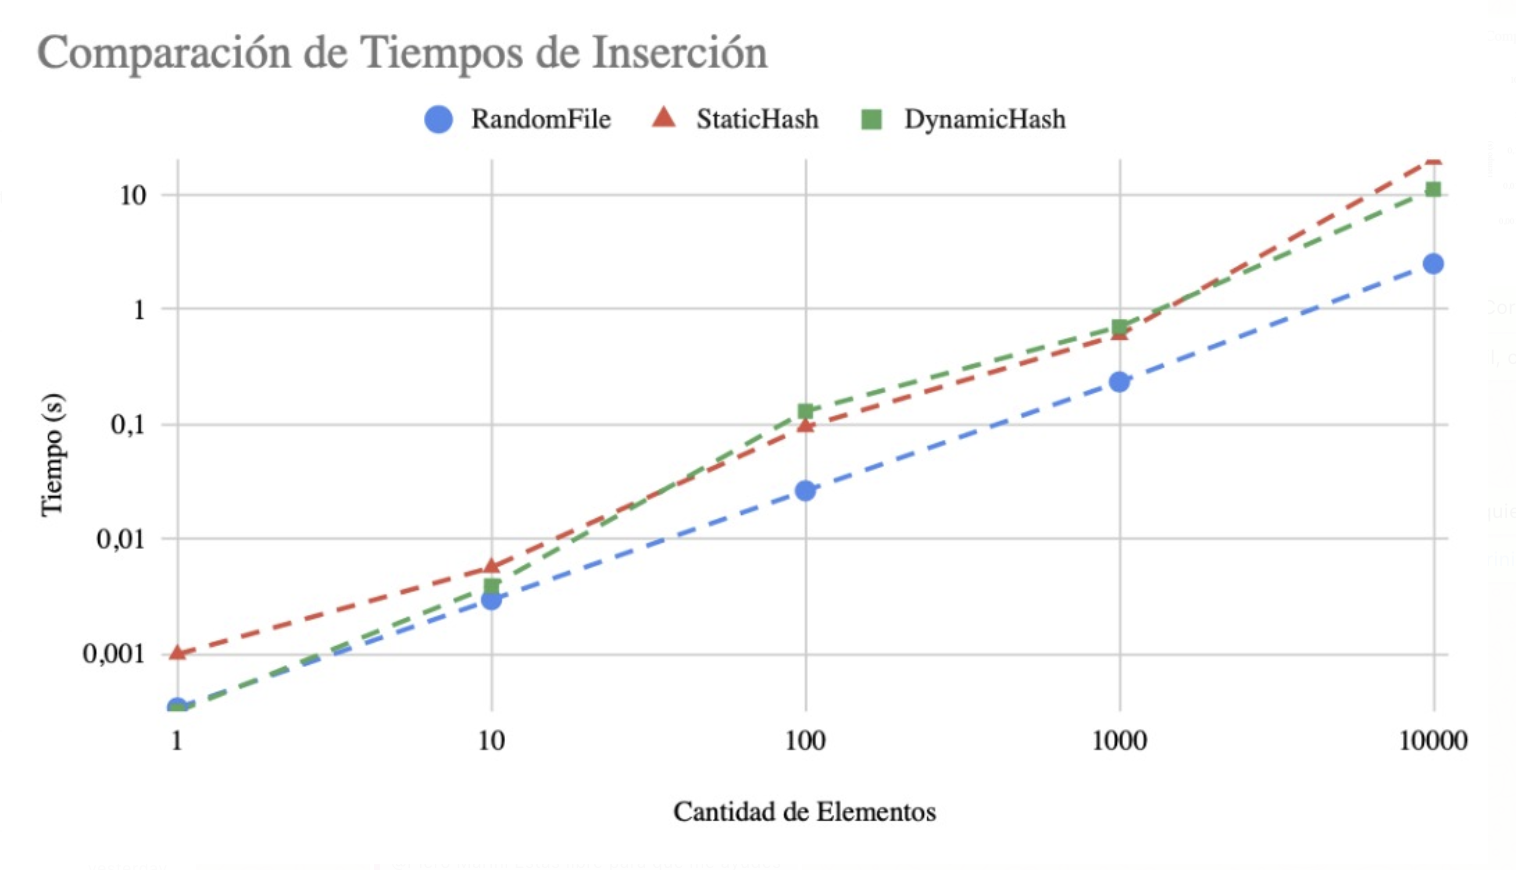
\includegraphics[width = \textwidth]{tiempoInsercion}
        \caption{Cuadro comparativo del tiempo de inserción de cada una de las técnicas de Organización de Archivos}

      \end{figure}

      \begin{figure}[h]

        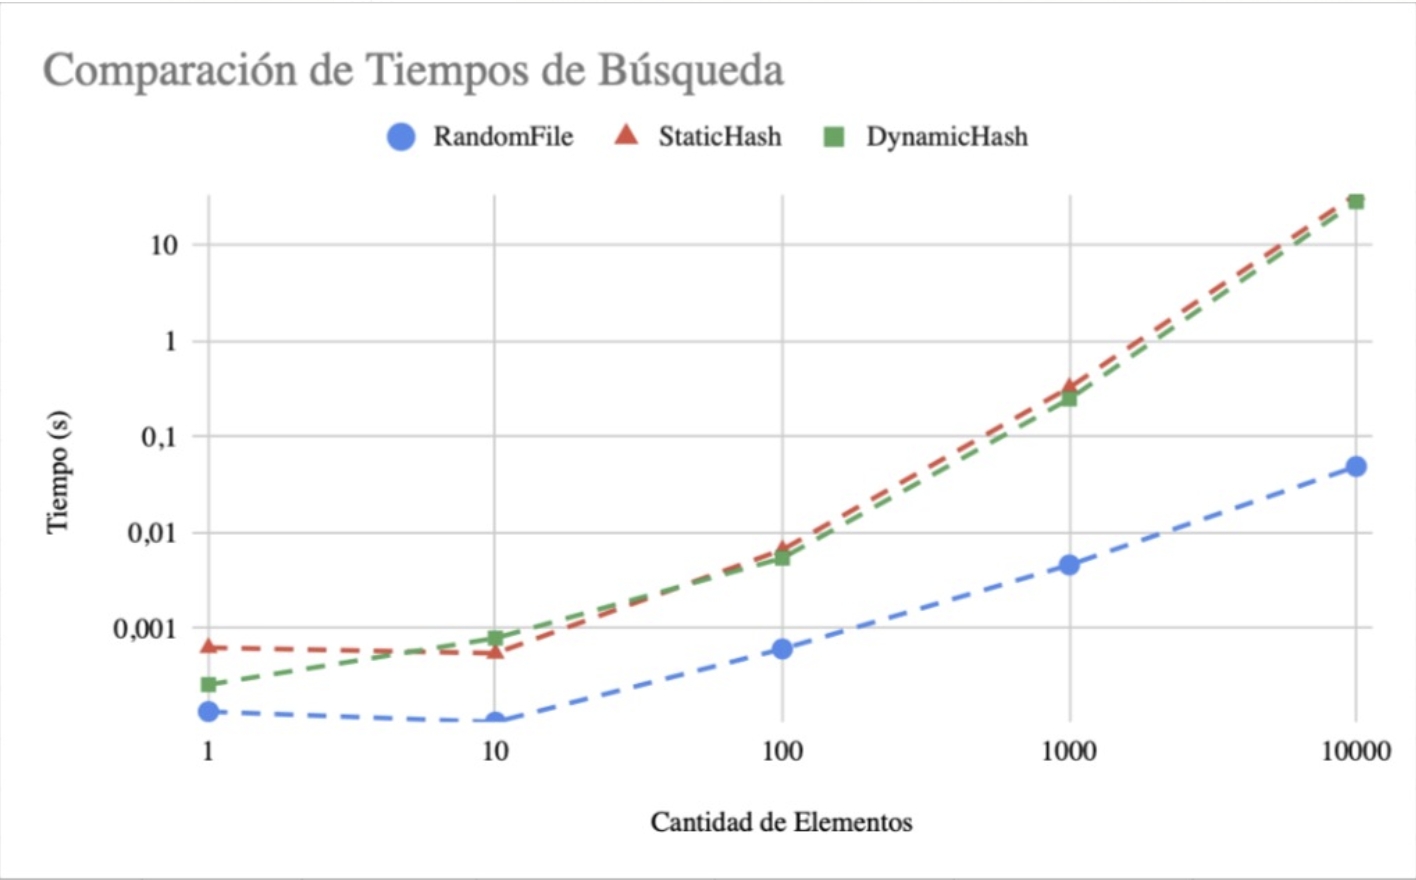
\includegraphics[width = \textwidth]{tiempoBusqueda}
        \caption{Cuadro comparativo del tiempo de búsqueda de caddad una de las técnicas de Organización de Archivos}

      \end{figure}

    \subsection{Análisis de los Resultados}

      Como es posible observar en los gráficos presentados, el tiempo de inserción y búsqueda tiende a ser mucho menor en el Random File Organization comparado con las otras técnicas de hasheo utilizadas. Esto se puede deber a que en este método de archivos carga todo su index en memoria primaria antes de empezar. En comparación, Static Hashing y Dynamic Hashing requieren estar constantemente haciendo accesos a disco más pequeños para recuperar el map que los lleva a determinado registro. Con respecto a estos últimos 2, el Static Hashing presenta pequeñas ventajas cuando se refiere a trabajar con pequeñas cantidades de datos, o una profundidad alta, debido a que los casos de overflow son mínimos. Sin embargo, conforme la cantidad de archivos a insertarse y/o buscarse aumentaba, se veían claras mejoras en el uso de Dynamic Hashing. Las diferencias de tiempo se hacían exponenciales conforme el número de operaciones aumentaba. \\

      Las ventajas del dynamic hashing es que evita los overflows iniciales diviendo los buckets con una profundidad local menor en buckets de profundidad mayor. Un caso común que ocurría en las búsquedas finales  (de elementos que se encontraban casi al final de los buckets estáticos), es que se tenía que recorrer todos los buckets previos de forma secuencial, lo cual añadía sustancialmente al tiempo necesario para encontrar el registro necesario. En el caso del dynamic hashing, debido a la menor cantidad de buckets que se encuentran en desenbordamiento encadenado, no es necesario hacer un recorrido secuencial tan largo para llegar al registro en cuestión.

  \section{Pruebas de Uso}

    Como pruebas de uso de la aplicación creada fueron a través de transacciones que realizaban las operaciones básicas de la base de datos. Estas tenían diferentes iteraciones de las operaciones de inserción y búsqueda. Se tomaron las siguientes imagenes de la implementación y el funcionamiento de las mismas.

  \section{Conclusiones}
    
    Sintetizando, se pudieron analizar e implementar satisfactoriamente tres técnicas de organización de archivos para una base de datos relacional. Como fuente de información se utilizó una base de datos previamente existente, pero que sufría porblemas en su gestión debido a su planteamiento. El trabajo consistió en replantear esta base de datos para hacerla trabajable (además de crear una función de generación de datos aleatoria) y realizar operaciones en la misma a través de las técnicas implementadas. Las pruebas de uso a través de las transacciones se completaron de forma eficiente y mostraron un cierto nivel de control de concurrencia al ser ejecutadas en simúltaneo. En una futura iteración del proyecto se desea realizar una interfaz gráfica para realizar las operaciones. \\

    Las dificultades que surgieron durante el trabajo estan orientadas tanto a la limpieza de la base de datos original, como a la implementación de las diferentes técnicas. Por un lado, la falta de coherencia de la base de datos, hubieron complicaciones al momento de leer los archivos a variables de tamaño fijo para poder realizar las implementaciones. Este fue el motivo principal para hacer una función que genere datos aleatoriamente. Por otra parte, el trabajar con memoria secundaria complico las implementaciones de las técnicas de manejo de archivos, debido a que no se podía tener todo en memoria principal al mismo tiempo, fue necesario la creación de archivos de meetadata para guardar la información, lo cual represento un costo adicional para algunas de las operaciones. Un aspecto que resulto de guía fue el hacer una analogía entre \textit{filenames} y punteros, que se comportaban de manera similar en la organización de archivos. 
  
  \section{Anexo}
    
    \subsection{Link del Código en GitHub}

      https://github.com/DiegoELT/db2Project1.git

\end{document}
